\documentclass[a4paper, 12pt]{article}%тип документа

%отступы
\usepackage[left=2cm,right=2cm,top=2cm,bottom=3cm,bindingoffset=0cm]{geometry}

%Русский язык
\usepackage[T2A]{fontenc} %кодировка
\usepackage[utf8]{inputenc} %кодировка исходного кода
\usepackage[english,russian]{babel} %локализация и переносы

%Вставка картинок
\usepackage{wrapfig}
\usepackage{graphicx}
\graphicspath{{pictures/}}
\DeclareGraphicsExtensions{.pdf,.png,.jpg}

%оглавление
\usepackage{titlesec}
\titlespacing{\chapter}{0pt}{-30pt}{12pt}
\titlespacing{\section}{\parindent}{5mm}{5mm}
\titlespacing{\subsection}{\parindent}{5mm}{5mm}
\usepackage{setspace}

%Графики
\usepackage{multirow}
\usepackage{pgfplots}
\pgfplotsset{compat=1.9}

%Математика
\usepackage{amsmath, amsfonts, amssymb, amsthm, mathtools}

\begin{document}

\begin{titlepage}

\begin{center}
%\vspace*{1cm}
\large\textbf{Московский Физико-Технический Институт}\\
\large\textbf{(государственный университет)}
\vfill
\line(1,0){430}\\[1mm]
\huge\textbf{Петля гистерезиса (динамический метод)}\\
\line(1,0){430}\\[1mm]
\vfill
\large Сибгатуллин Булат, ФРКТ\\
\end{center}

\end{titlepage}

\section*{Цель работы}
Исследование предельных петель гистерезиса и начальных кривых намагничивания для нескольких ферромагнитных образцов; определение магнитных характеристик материалов, чувствительность каналов $X$ и $Y$ осциллографа и постоянную времени $\tau$ интегрирующей цепочки.
\section*{В работе используются}
автотрансформатор, понижающий трансформатор, амперметр и вольтметр, резистор, делитель напряжения, интегрирующая цепочка, электронный осциллограф, тороидальные образцы с двумя обмотками.
\section*{Экспериментальная установка}
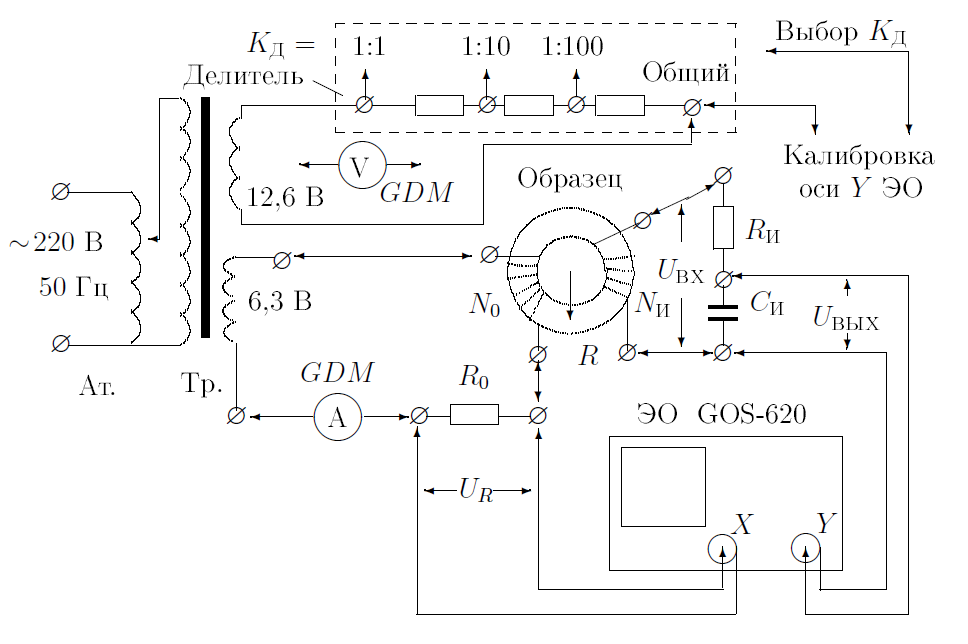
\includegraphics[width = \textwidth]{1.png}

Действующее значение переменного тока в обмотке $N_0$ измеряется амперметром $A$. Последовательно с амперметром включено сопротивление $R_0$, напряжение с которого подается на вход $X$ электронного осциллографа. Это напряжение пропорционально току в обмотке $N_0$, а следовательно и напряженности $H$ магнитного поля в образце.

Для измерения магнитной индукции $B$ с измерительной обмотки $N_{\textit{и}}$ на вход интегрирующей $RC$-цепочки подается напряжение $U_{\text{и}}(U_{\textit{вх}})$, пропорциональное $\dot{B}$, а, с выхода снимается напряжение $U_{\textit{с}}(U_{\textit{вых}})$, пропорциональное величине $B$, а подается на вход $Y$.

\section*{Теория}
\subsection*{Измерение напряжения с помощью осциллографа}
Исследуемый сигнал подается на вход $X$; длина $2x$ горизонтальной черты, наблюдаемой на экране, характеризует удвоенную амплитуду сигнала. 

Если известна чувствительность усилителя $K_x$ в вольтах на деление шкалы экрана, то удвоенная амплитуда напряжения определяется произведением
\[2U_{X, 0} = 2x \cdot K_x\]
Напряжение, подаваемое на вход $Y$ определяется аналогично. 

Калибровку осей осциллографа можно использовать для построения кривой гистерезиса в координатах $B$ и $H$:

Зная величину сопротивления $R_0$, с которого снимается сигнал, можно определить чувствительность канала по току $K_{XI} = \dfrac{K_x}{R_0}$ [A/дел]; затем, используя формулу 
\begin{equation}
H = \dfrac{IN_0}{2\pi R}
\end{equation}
определить цену деления шкалы в A/м.

Используя формулу 
\begin{equation}
B = \dfrac{R_{\text{и}}C_{\text{и}}U_{\text{вых}}}{SN_{\text{и}}}
\end{equation}
можно рассчитать цену деления вертикальной шкалы в теслах.
\subsection*{Проверка калибровки горизонтальной оси ЭО с помощью амперметра}
проводится при закороченной обмотке $N_0$. Эта обмотка с помещенным в нее ферромагнитным образцом является нелинейным элементом, так что ток в ней не имеет синусоидальной формы, и это не позволяет связать амплитуду тока с показаниями амперметра.
\begin{equation}
m_X = \dfrac{2 \sqrt{2} R_0 I_{\text{эф}}}{2x} \text{[B/дел]}
\end{equation}
\subsection*{Проверка калибровки вертикальной оси ЭО с помощью вольтметра}
Сигнал с обмотки 12,6 В понижающего трансформатора подается на делитель напряжения. Часть этого напряжения снимается с делителя с коэффициентом деления $K_{\text{Д}}$ (1/10 или 1/100) и подается на вход $Y$. Мультиметр $V$ измеряет напряжение $U_{\text{эф}}$ на этих же клеммах делителя.

Далее по формуле 
\begin{equation}
m_Y = \dfrac{2\sqrt{2}U_{\text{эф}}}{2y} \text{[B/дел]}
\end{equation}
можно рассчитать чувствительность канала $Y$.
\subsection*{Постоянная времени $RC$-цепочки}
Рассчитывается по формуле 
\begin{equation}
RC = \dfrac{U_{\text{вх}}}{\Omega U_{\text{вых}}}
\end{equation}

\section*{Задание}
\subsection*{Измерение петли гистерезиса}

\begin{enumerate}

\item Соберем схему экспериментальной установки. Подберем ток питания в намагничивающей обмотке, так чтобы на экране ЭО наблюдалась предельная петля гиперэкстезиса. Сфотографируем данную картину и запишем значения коэффициентов усиления $K_x$ и $K_y$ осциллографа и действующее значение тока \textit{I} в намагничивающей обмотке.

\item По экрану ЭО измерим полную ширину и высоту ([$2X_s$] и [$2Y_s$]), соответствующие удвоенной амплитуде колебания напряженности $H_s$ и индукции $B_s$ поля в образце в состоянии насыщения.

\item По экрану ЭО измерим двойные амплитуды для коэрцитивного поля [$2X_c$] и остаточной индукции [$2Y_r$].

\item Процедем измерение начальной кривой намагничивания. Плавно уменьшая амплитуду намагничивания до нуля, будем фиксировать по экрану осциллографа положения крайних точек, наблюдаемых частных петель. Запишем материал образца и параметры тороида.

\item Повторим измерения пп. 1-4 для остальных катушек.

\subsection*{Калибровка осциллографа}

\item Проведем калибровку горизонтальной оси осциллографа, для этого не разбирая экспериментальную установку <<закоротим>>  намагничивающую обмотку $N_0$.

Измерим длину наблюдаемой развертки по оси \textit{X}, при некотором фиксированном токе \textit{I}, близком к току насыщения петли гистерезиса. Проведем измерения для всех значений $K_x$, использовавшихся в работе.

\item Для проверки калибровки вертикальной оси ЭО подключим вольтметр и осциллограф к делителю 1:100 и сравним показания вольтметра и осциллографа. Оценим погрешность измерений амплитуды с помощью осциллографа.

\subsection*{Определение параметров \textit{RC}-ячейки}

\item Измерим постоянную времени \textit{RC}-ячейки $\tau_{\textit{и}}$. Измерим отношение входного и выходного напряжений $U_{\textit{вх}}/U_{\textit{вых}}$ ячейки с помощью осциллографа. Рассчитаем постоянную времени.

\item Сравним результат с расчетом непосредственно через $R_{\textit{и}}$ и $_{\textit{и}}$, указанными на установке. 

\end{enumerate}

\section*{Ход работы}

\subsection*{Петля гистерезиса}

\begin{center}
\begin{tabular}{|c|c|c|c|}
\hline 
 & Пермаллой & Феррит & Кремнистое железо \\ 
\hline 
$N_0, \: \textit{витков}$ & 40 & 35 & 35 \\ 
\hline 
$N_{\textit{И}}, \: \textit{витков}$ & 200 & 400 & 350 \\ 
\hline 
$S, \: \textit{см}^2$ & 3,8 & 3 & 1,2 \\ 
\hline 
$2\pi r, \: \textit{см};$ & 24 & 25 & 10 \\ 
\hline 
\end{tabular}

\textbf{Таблица 1.} Некоторые характеристики образцов.
\end{center}

Запишем параметры установки.

\begin{center}
\begin{tabular}{|c|c|}
\hline 
$R_0, \: \textit{Ом}$ & 0,3 \\ 
\hline 
$R_{\textit{И}}, \: \textit{Ом}$ & 20 \\ 
\hline 
$C_{\textit{И}}, \: \textit{мкФ}$ & 20 \\ 
\hline 
\end{tabular} 

\textbf{Таблица 2.} Некоторые параметры установки.
\end{center}

\begin{center}
\begin{tabular}{|c|c|c|c|c|c|c|}
\hline
 & Величина & $\sigma$ & Величина & $\sigma$ & Величина & $\sigma$ \\ \hline
 & \multicolumn{2}{c|}{Пермаллой} & \multicolumn{2}{c|}{Феррит 1000нн} & \multicolumn{2}{c|}{Кремнистое железо} \\ \hline
Петля & \multicolumn{2}{c|}{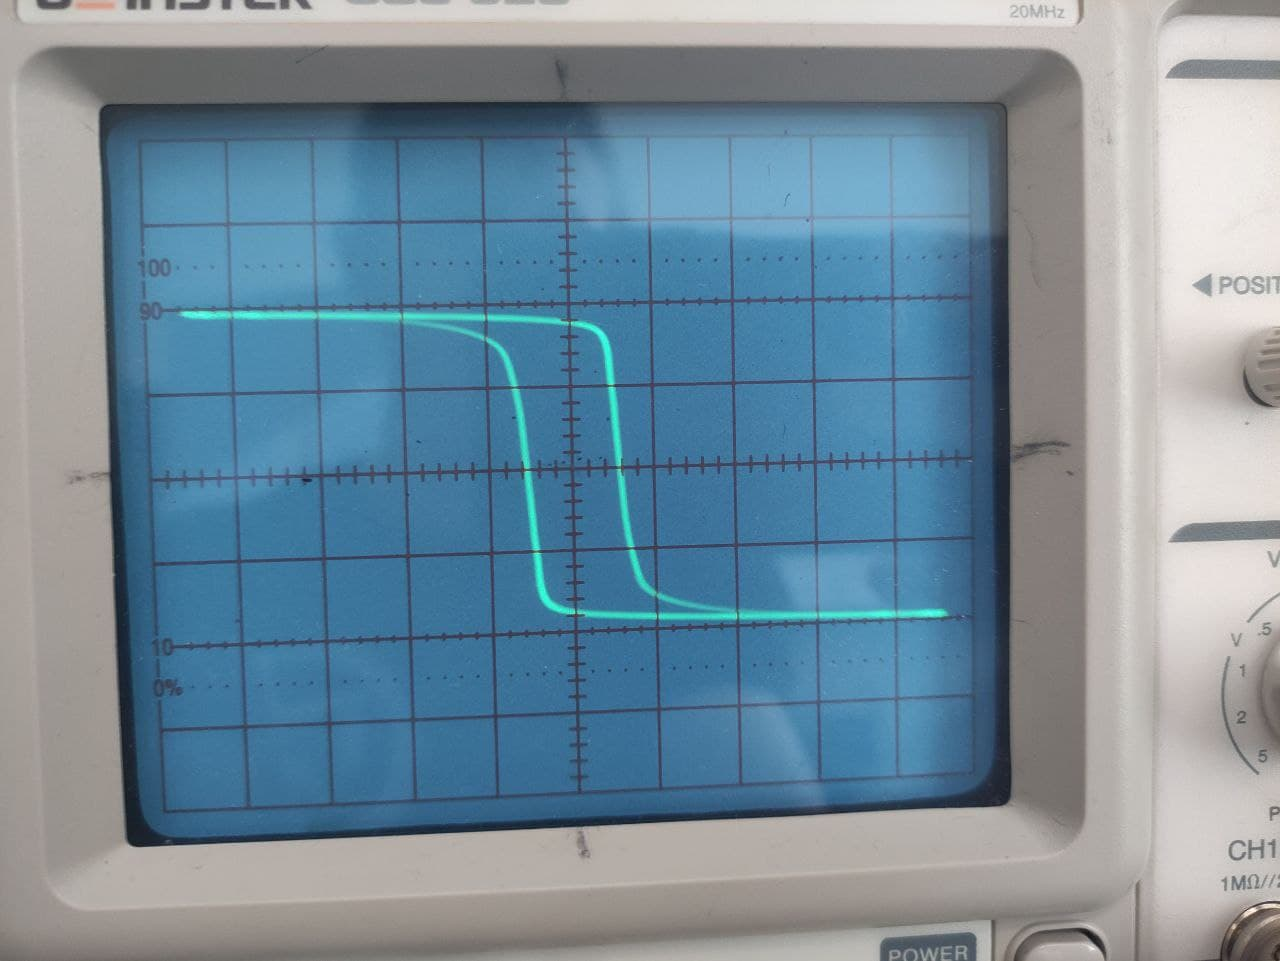
\includegraphics[width = 0.2\textwidth]{Пермаллой.jpg}} &  \multicolumn{2}{c|}{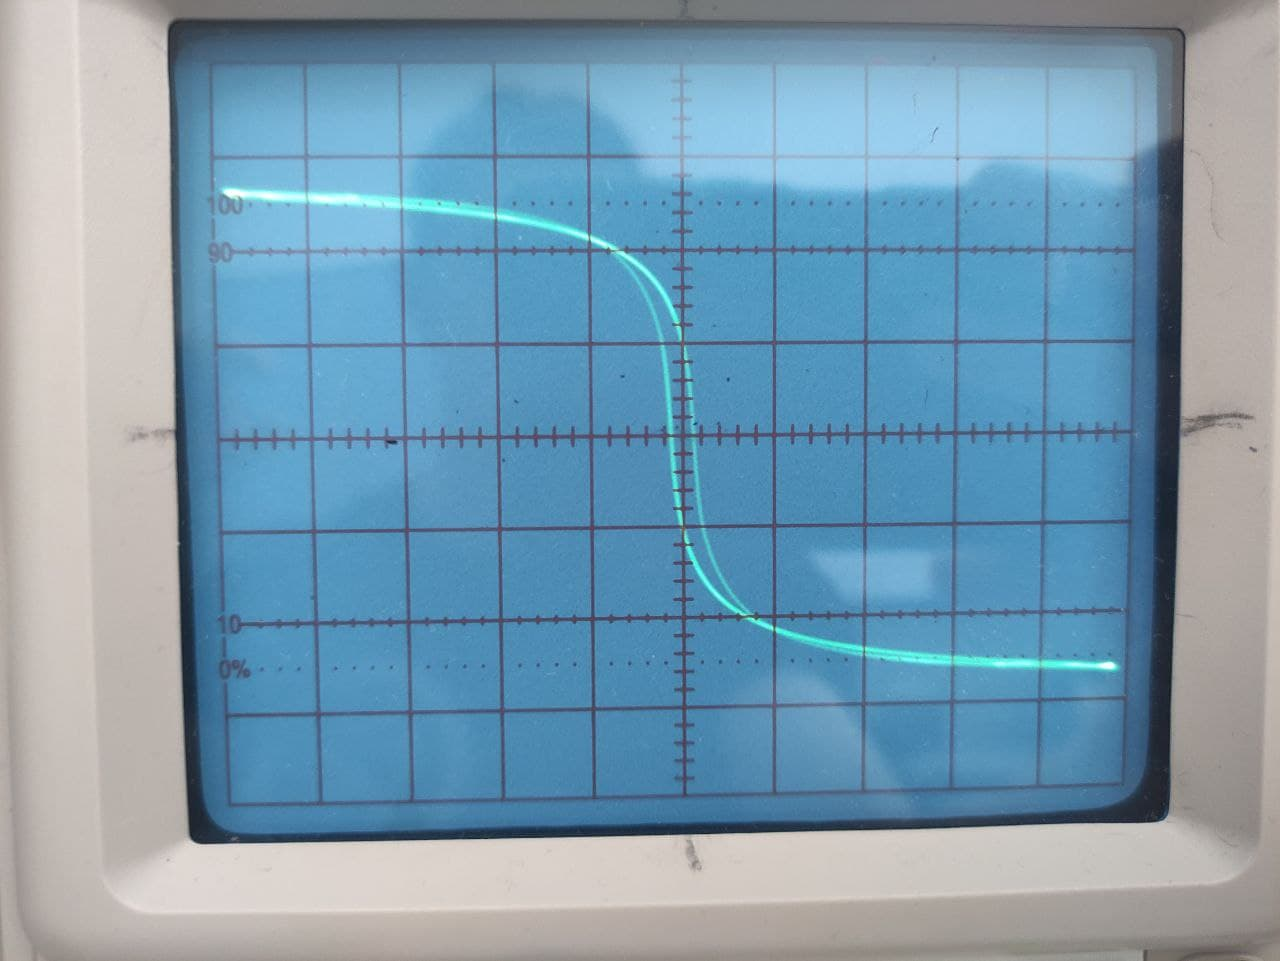
\includegraphics[width = 0.2\textwidth]{Феррит.jpg}} &  \multicolumn{2}{c|}{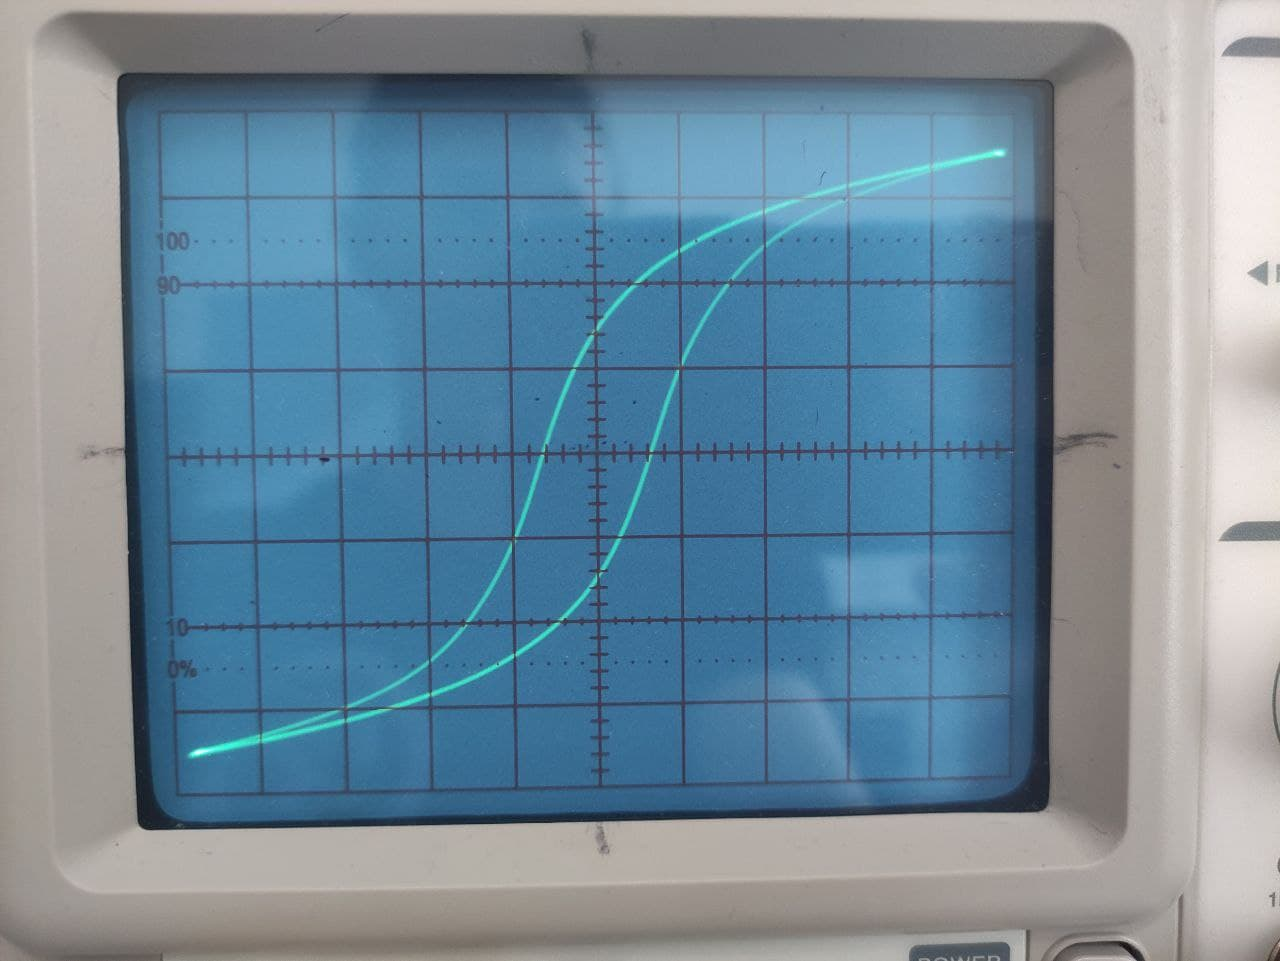
\includegraphics[width = 0.2\textwidth]{Кремнистое_железо.jpg}} \\ \hline
$I_{\text{эф}}$, А & 0,690 & 0,001 & 1,060 & 0,001 & 1,000 & 0,001 \\ \hline
$[2x(c)]$, ед & 9,2 & 0,2 & 10,0 & 0,2 & 9,6 & 0,2 \\ \hline
$[2y(s)]$, ед & 4,0 & 0,2 & 5,2 & 0,2 & 7,2 & 0,2 \\ \hline
$K_x$, мВ/дел & 100 & 0 & 100 & 0 & 100 & 0 \\ \hline
$K_y$, мВ/дел & 100 & 0 & 20 & 0 & 50 & 0 \\ \hline
$H$, (А/м)/дел & 0,556 & 0 & 0,467 & 0 & 1,167 & 0 \\ \hline
$H_c$, А/м & 5,12 & 0,11 & 4,67 & 0,09 & 11,21 & 0,23 \\ \hline
$B$, Тл/дел & 0,526 & 0 & 0,067 & 0 & 0,476 & 0 \\ \hline
$B_s$, Тл & 2,11 & 0,11 & 0,347 & 0,013 & 3,42 & 0,09 \\ \hline
\end{tabular}\\

\textbf{Таблица 3.} Данные, полученные из петли гистерезиса.
\end{center}

\subsection*{Проверка калибровки оси X}

Отключаем намагничивающую обмотку от цепи, соединив оба провода, идущих к обмотке, на одной из ее клемм. 

Подбираем такой ток, чтобы горизонтальная прямая занимала большую часть экрана.

Рассчитаем чувствительность канала $m_X$ по формуле $(3)$. 

Результаты смотри в таблице 4.

\subsection*{Проверка калибровки оси Y}

Разберем цепь. Соединим вход $Y$ с клеммами делителя "1/100-земля". Не меняя рабочего коэффициента $K_Y$, подберем с помощью трансформатора напряжение, при котором вертикальная прямая занимает почти весь экран. Измеряем длину $2y$. Запишем данные из двух вышеизложенных пунктов в таблицу. Рассчитаем $m_Y$ по формуле $(4)$.

\begin{center}
\begin{tabular}{|c|c|c|}
\hline 
 & Величина & $\sigma$ \\  
\hline 
$m_X$, [В/дел] & 0,092 & 0,002 \\ 
\hline 
$K_X$, [В/дел] & 0,1 & 0 \\ 
\hline 
$m_Y$, [В/дел] & 0,0198 & 0,0004 \\ 
\hline 
$K_Y$, [В/дел] & 0,02 & 0 \\ 
\hline 
$m_Y$, [В/дел] & 0,0964 & 0,0006 \\ 
\hline 
$K_Y$, [В/дел] & 0,1 & 0 \\ 
\hline 
\end{tabular}
 
\textbf{Таблица 4.} Калибровка осей осциллографа.
\end{center}

По таблице видим, что соответствующие $K$ и $m$ равны с точностью до погрешности.

\subsection*{Расчет $\tau$ постоянной времени для цепочки}

Запишем все полученные данные в таблицу и посчитаем $\tau$ по формуле $(5)$ и через параметры установки.

\begin{center}
\begin{tabular}{|c|c|c|}
\hline 
 & Значение & Ошибка \\ 
\hline 
$U_{\text{вх}}$, В & 6,5 & 0,2 \\ 
\hline 
$U_{\text{вых}}$, В & 0,048 & 0,002 \\ 
\hline 
$\tau_{\text{теор}}$, с & 0,43 & 0,02 \\ 
\hline 
$\tau_{\text{эксп}}$, с & 0,40 & 0 \\ 
\hline 
\end{tabular} 

\textbf{Таблица 5.} Измерение $\tau$.
\end{center}

\subsection*{Начальный кривые намагничивания}

Зарисуем графики начальных кривых намагничивания для наших образцов.

\begin{figure}[h!]
\centering
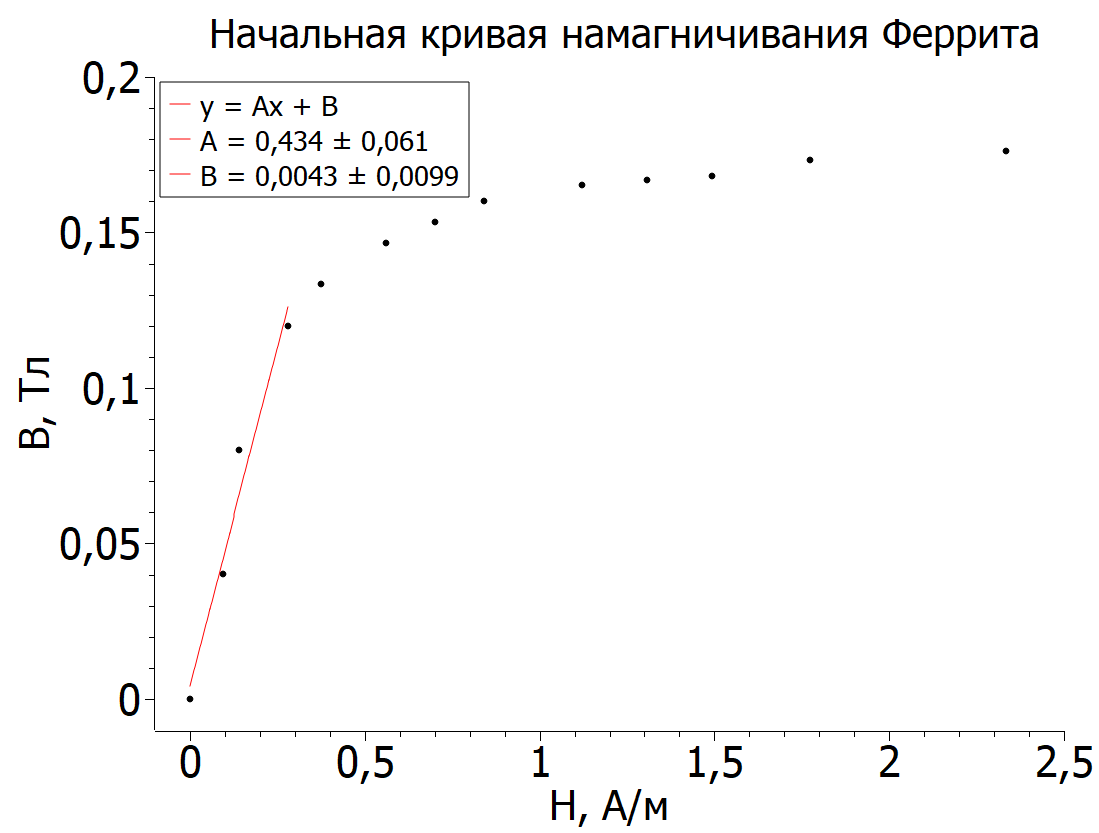
\includegraphics[scale=0.5]{Феррит.png}
\label{fig:Image1}
\end{figure}

\begin{figure}[h!]
\centering
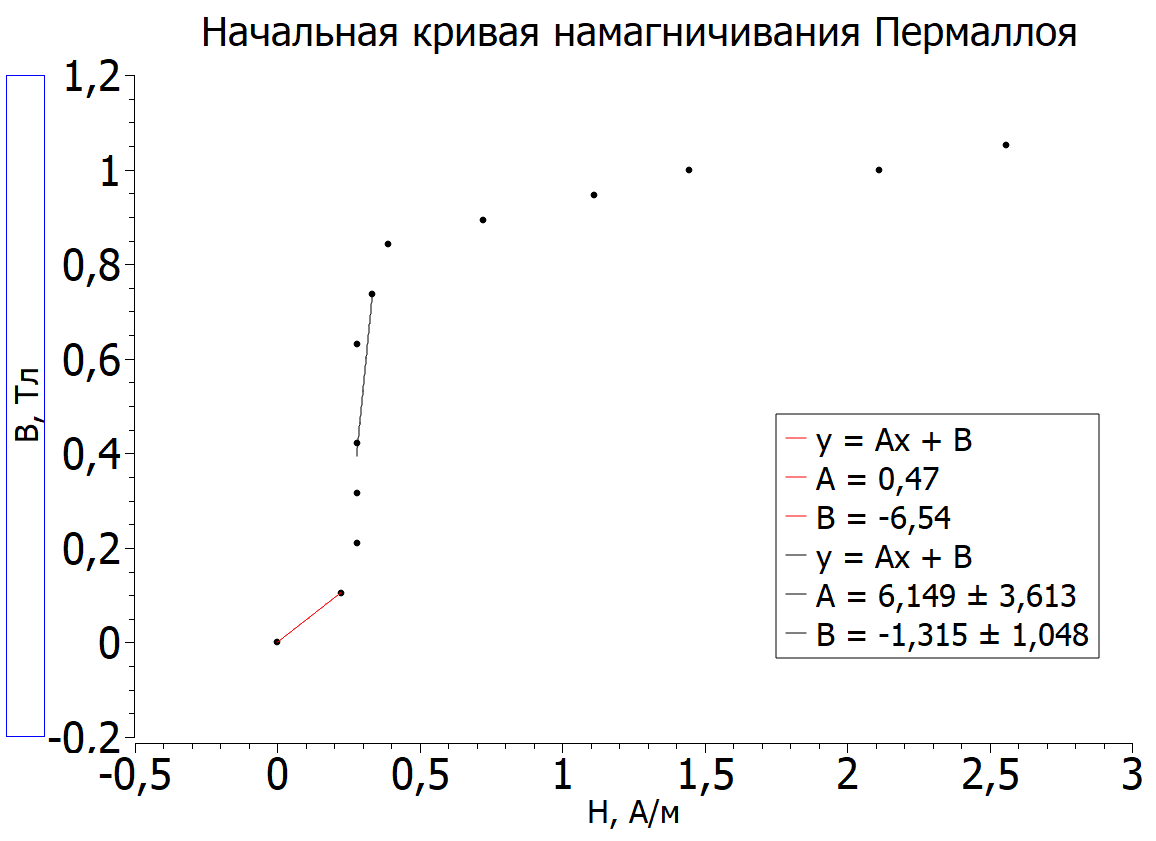
\includegraphics[scale=0.5]{Пермаллой.png}
\label{fig:Image1}
\end{figure}

\begin{figure}[h!]
\centering
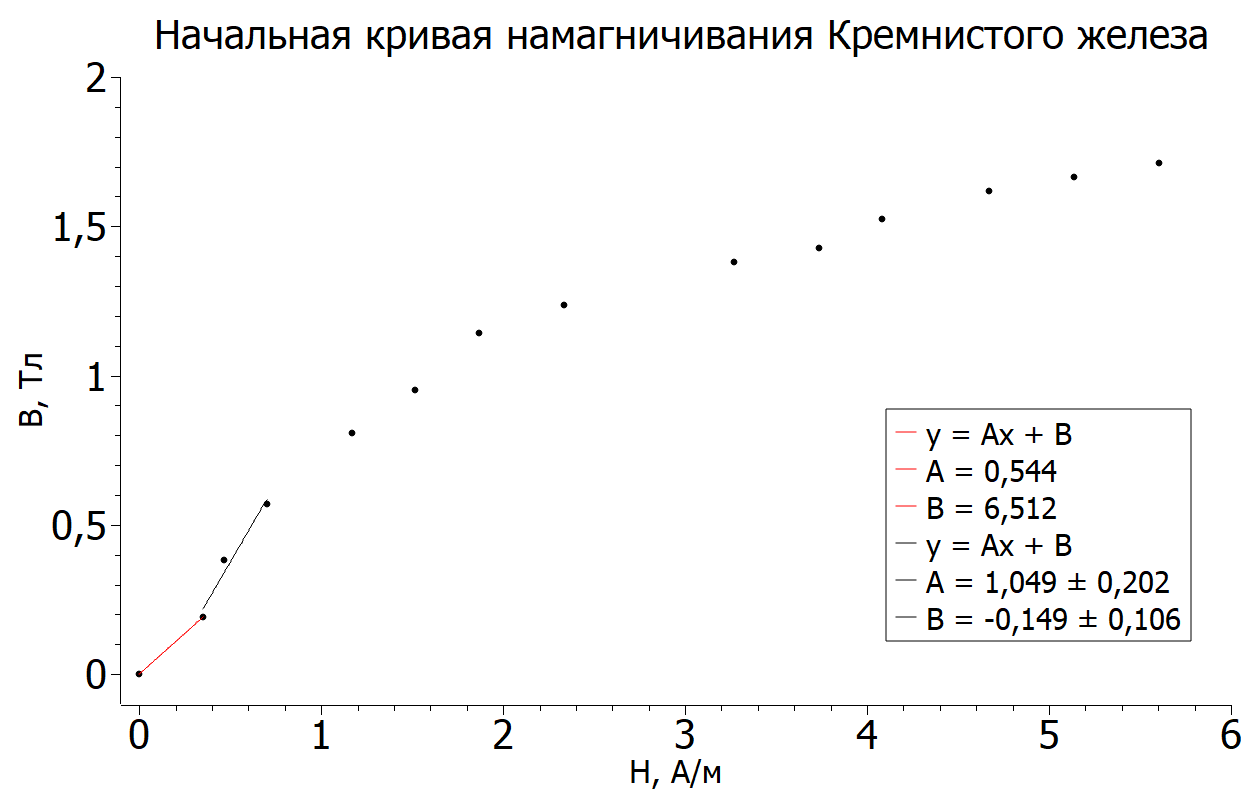
\includegraphics[scale=0.5]{Кремнистое_железо.png}
\label{fig:Image1}
\end{figure}

По графикам определим $\mu_{\text{диф}} = dB/dH$. Значения для $\mu_{\text{диф}}$ запишем прямо на графиках. Красная прямая будет отражать начальное значение дифференциальной магнитной проницаемости, а черная максимальное значение. Для Феррита начальное и максимальное значение совпадают.

Сравним $H_c$, $B_s$ и $\mu_{\text{диф}}$ с табличными.

\begin{center}
\begin{tabular}{|c|c|c|c|c|}
\hline
 & Ампл. & Fe-Ni & Fe-Si & Феррит \\ \hline
эксп & \multirow{2}{*}{$H_c$, A/м} & $5,12 \pm 0,11$ & $11,21 \pm 0,23$ & $4,67 \pm 0,09$ \\ \cline{1-1} \cline{3-5} 
табл &  & 5,6 & 12 & 4-100 \\ \hline
эксп & \multirow{2}{*}{$B_s$, Тл} & $2,11 \pm 0,11$ & $3,42 \pm 0,09$ & $0,347 \pm 0,013$ \\ \cline{1-1} \cline{3-5} 
табл &  & 1,6 & 2,01 & 0,3-0,4 \\ \hline
эксп & \multirow{2}{*}{$\mu_{\text{нач}}$} & $0,47 \pm 0,03$ & $0,544 \pm 0,018$ & $0,434 \pm 0,064$ \\ \cline{1-1} \cline{3-5} 
табл &  & $1,2\cdot 10^3$ & $9\cdot 10^3$ & $10-2000$ \\ \hline
эксп & \multirow{2}{*}{$\mu_{\text{макс}}$} & $6,149 \pm 0,347$ & $6,512 \pm 0,209$ & $0,434 \pm 0,064$ \\ \cline{1-1} \cline{3-5} 
табл &  & $3,5\cdot 10^3$ & $4\cdot 10^4$ & $10-2000$ \\ \hline
\end{tabular}\\
\textbf{Таблица 6.} Сверка с табличными значениями.
\end{center}

\end{document}